\section*{Aufgabe 1}

Das Runge-Kutta-Verfahren 4. Ordnung wird für die Newtonschen Bewegungsgleichungen eines beliebigen Kraftfeldes untersucht
\begin{align*}
\dot{\vec{x}} &= \vec{v}\\
\dot{\vec{v}} &= \frac{\vec{F}(\vec{r})}{m}
\end{align*}
\subsection*{a)+b)}
Es wird für einen harmonischen Oszillator $\vec{F}= -\vec{r}m\omega^2$ mit Frequenz $\omega=1$ der Ort der Masse nach den ersten 10 Schwingungen und die Abweichung vom Startwert $|\vec{r}_i-\vec{r}_0|$ bei verschiedenen Schrittweiten bestimmt.
Die Abbildungen \ref{fig:1} und \ref{fig:2} zeigen die Toleranz in Abhängigkeit von der Schwingung bei den Anfangsbedingungen
\begin{equation}
\vec{r}_0 = \begin{pmatrix}
42\\
42\\
42
\end{pmatrix}, \vec{v}_0 = \vec{0}\label{eq:1}
\end{equation}
und
\begin{equation}
\vec{r}_0 = \begin{pmatrix}
42\\
42\\
42
\end{pmatrix}, \vec{v}_0 = \begin{pmatrix}
0\\
1\\
0
\end{pmatrix}\label{eq:2}
\end{equation}
Es zeigt sich, dass mit zunehmender Zeit die Bestimmung des Ortes schlechter wird. Um eine Toleranz von $10^{-5}$ erreichen, wird für die 1. Anfangsbedingung eine Schrittweite $h \leq 10^{-3}$ benötigt, während bei der 2. $h \leq 10^{-6}$ erforderlich ist.

\begin{figure}[h]
\centering
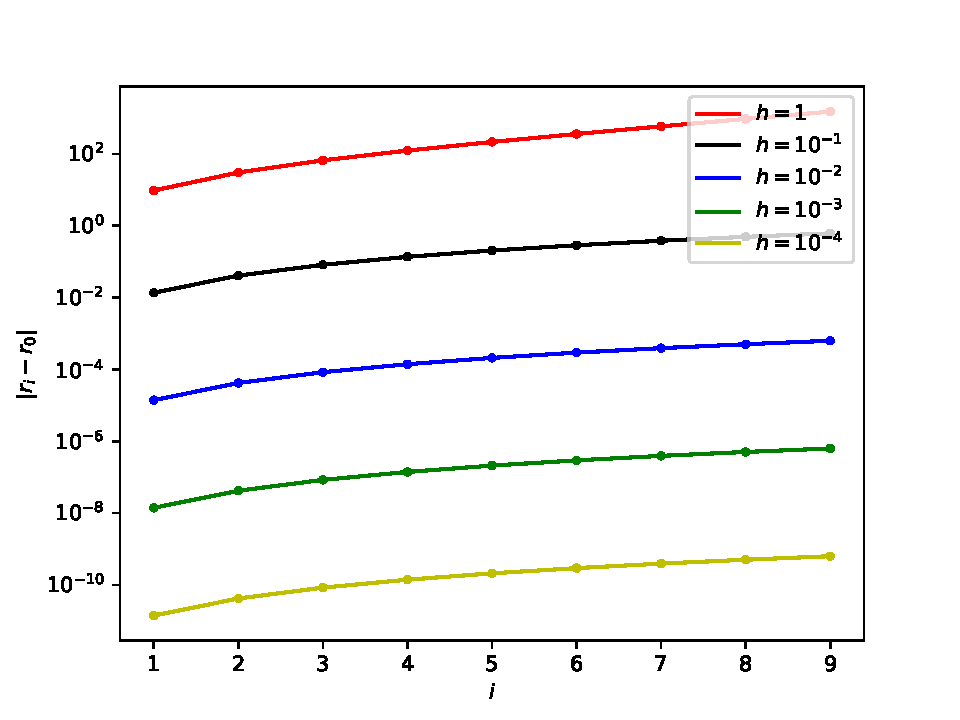
\includegraphics[width=0.75\textwidth]{A1/build/ab_plot.pdf}
\caption{Toleranz bei Anfangsbedingung \eqref{eq:1}.}
\label{fig:1}
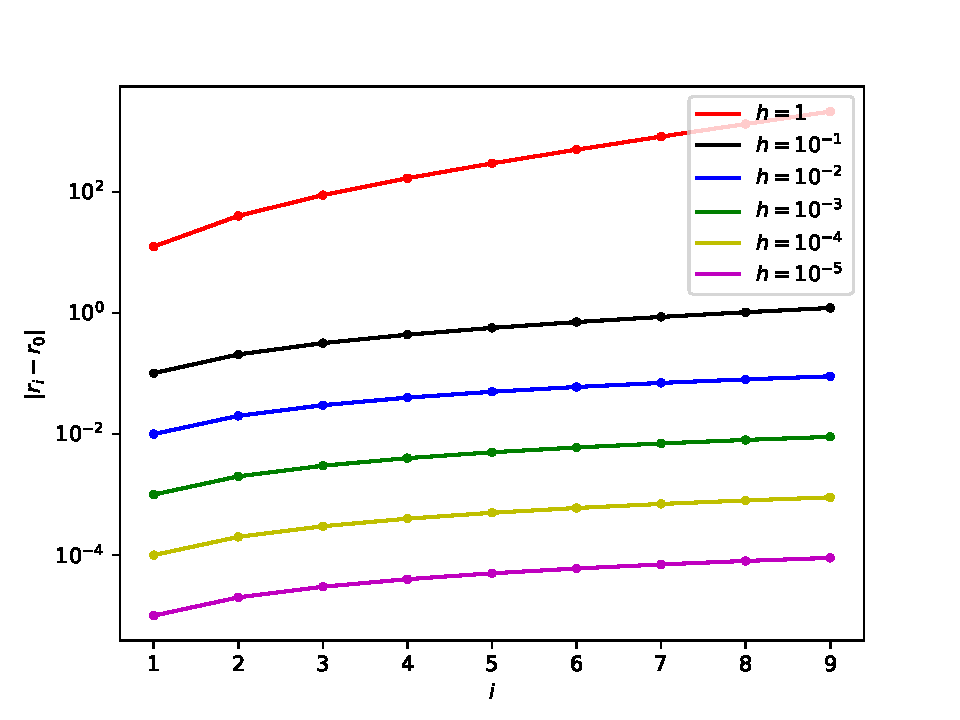
\includegraphics[width=0.75\textwidth]{A1/build/ab_plot2.pdf}
\caption{Toleranz bei Anfangsbedingung \eqref{eq:2}.}
\label{fig:2}
\end{figure}

\FloatBarrier

\subsection*{c)}
In Abbildung \ref{fig:3} ist die Abweichung von der Energie des Anfangszustandes nach $i$ Iterationen bei AB\eqref{eq:1} für $h=10^{-3}$ und $h=10^{-4}$ aufgetragen.
Anhand von Abbildung \ref{fig:1} ist ersichtlich, dass die Abweichung bei $h=10^{-4}$ um drei Größenordnungen kleiner und liegt unterhalb von $10^{-10}$. Dies führt dazu, dass auch die Energie genauer bestimmt werden kann. In Abb.\ref{fig:3} äußert sich das darin, dass für diese Schrittweite die Energieerhaltung gilt, während eine größere Schrittweite dies nicht gewährleistet.
\begin{figure}[h]
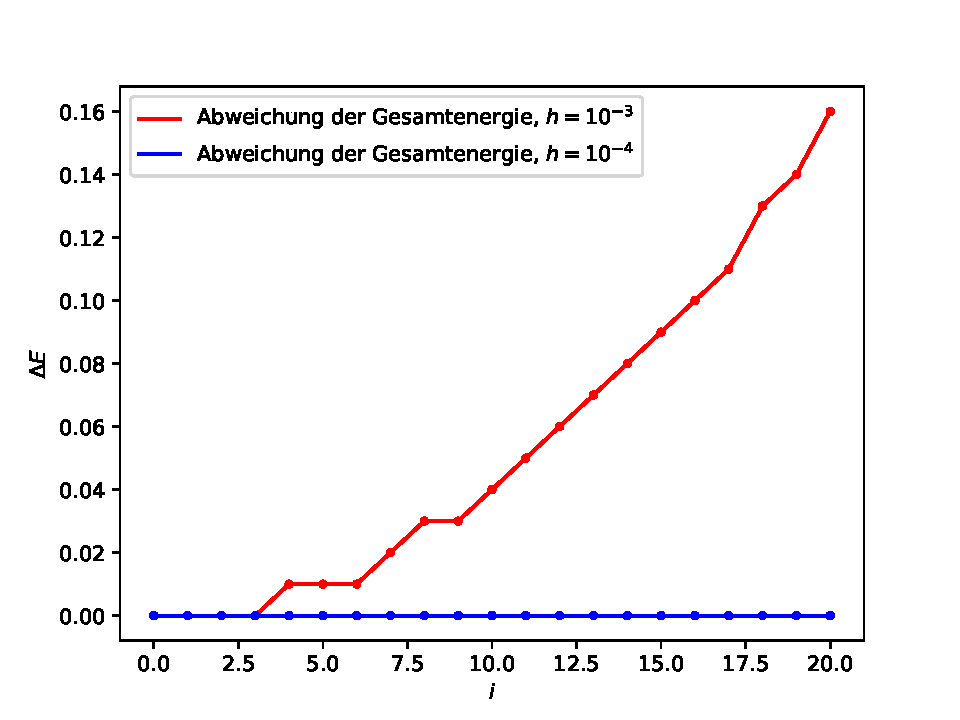
\includegraphics[width=0.8\textwidth]{A1/build/E.pdf}
\caption{Abweichungen von der Gesamtenergie mit AB\eqref{eq:1}.}
\label{fig:3}
\end{figure}